\chapter{Ethernet LAN Switching: Part
1}\label{ethernet-lan-switching-part-1}

\begin{figure}
\centering
\pandocbounded{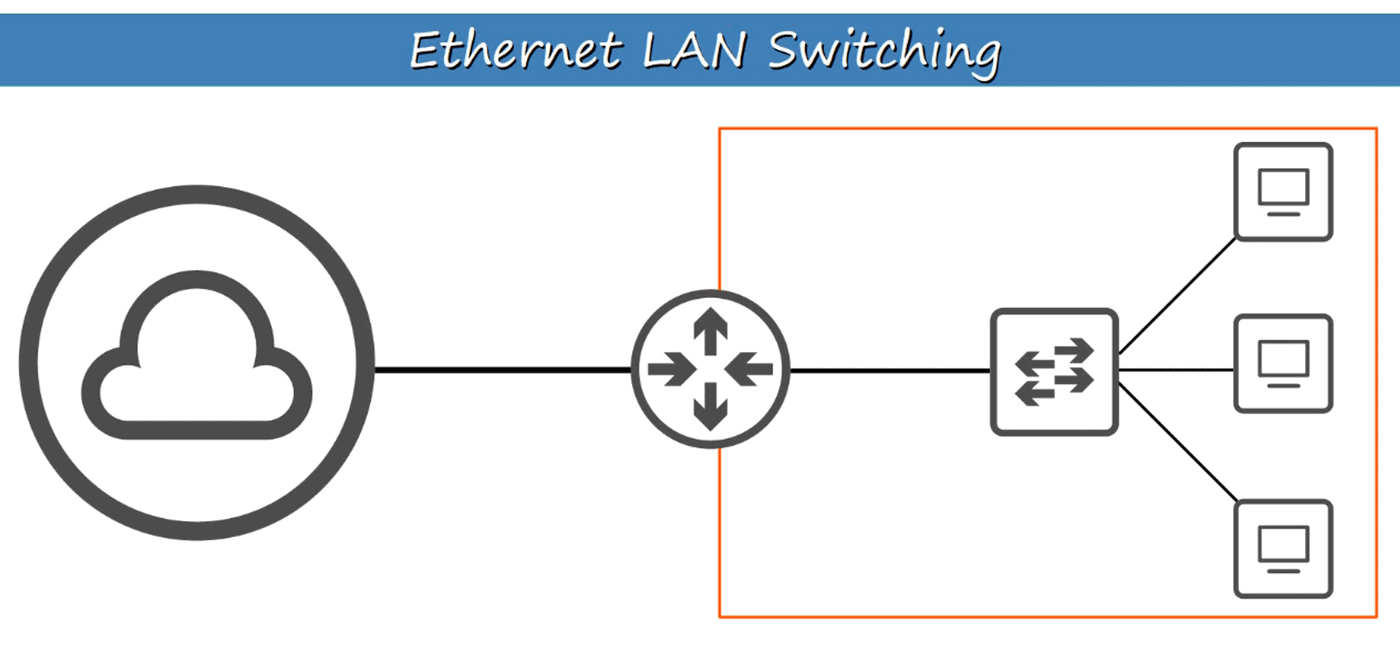
\includegraphics[keepaspectratio,alt={image}]{images/05-ethernet-lan-switching-part1/img-001.png}}
\end{figure}

\begin{figure}
\centering
\pandocbounded{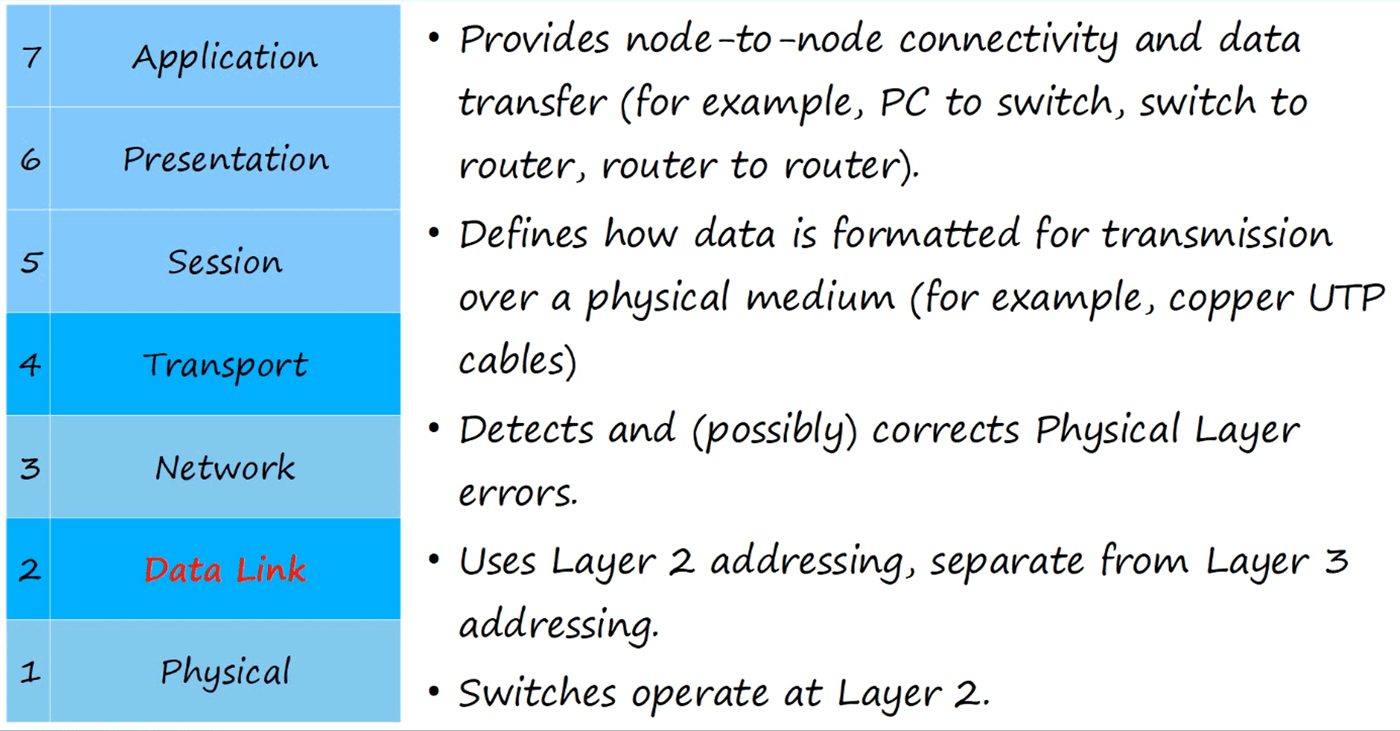
\includegraphics[keepaspectratio,alt={image}]{images/05-ethernet-lan-switching-part1/img-002.png}}
\end{figure}

LAN's

\begin{itemize}
\tightlist
\item
  A LAN is a network contained in a relatively small area.
\item
  Routers are used to connect separate LAN's
\end{itemize}

\begin{figure}
\centering
\pandocbounded{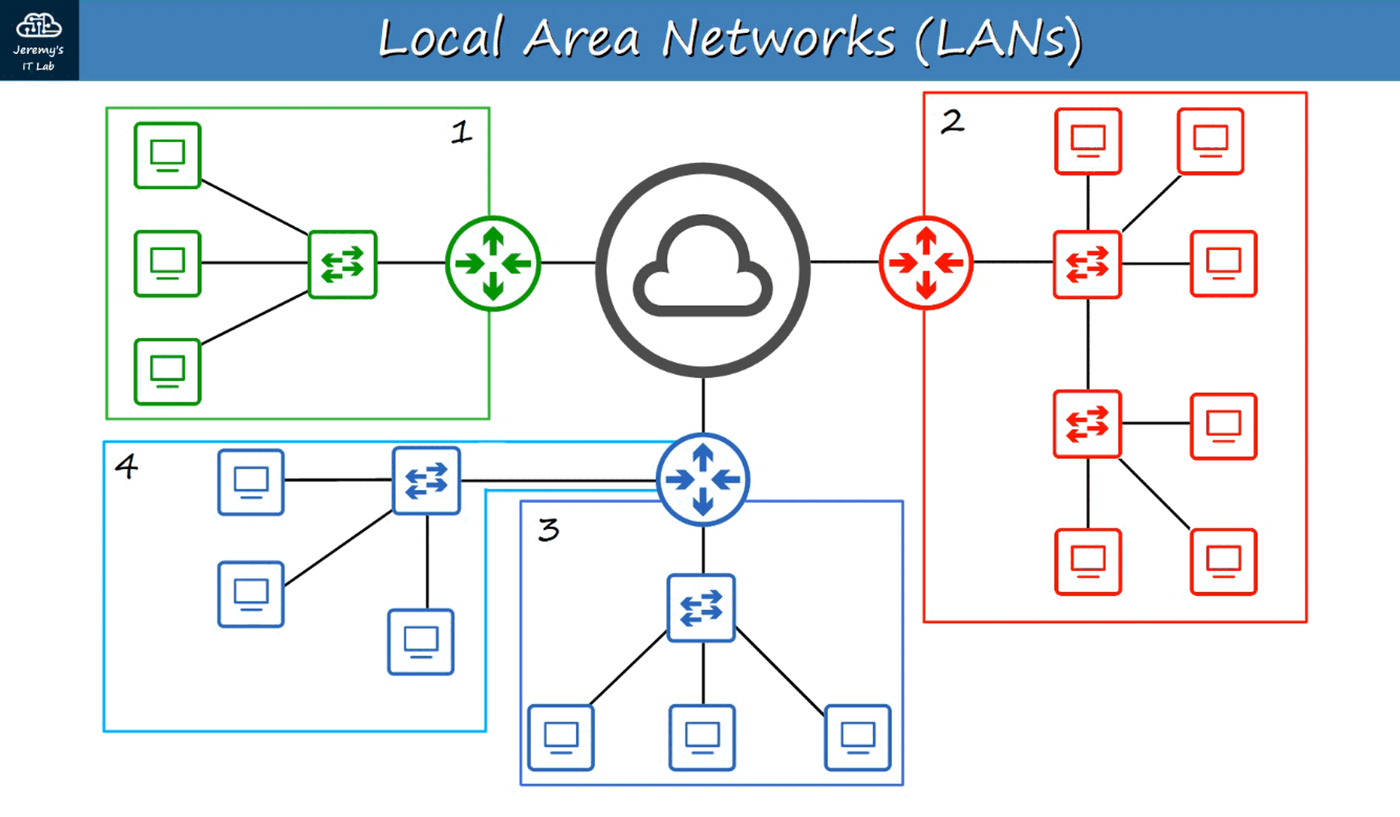
\includegraphics[keepaspectratio,alt={image}]{images/05-ethernet-lan-switching-part1/img-003.png}}
\end{figure}

An ETHERNET FRAME looks like:

\begin{figure}
\centering
\pandocbounded{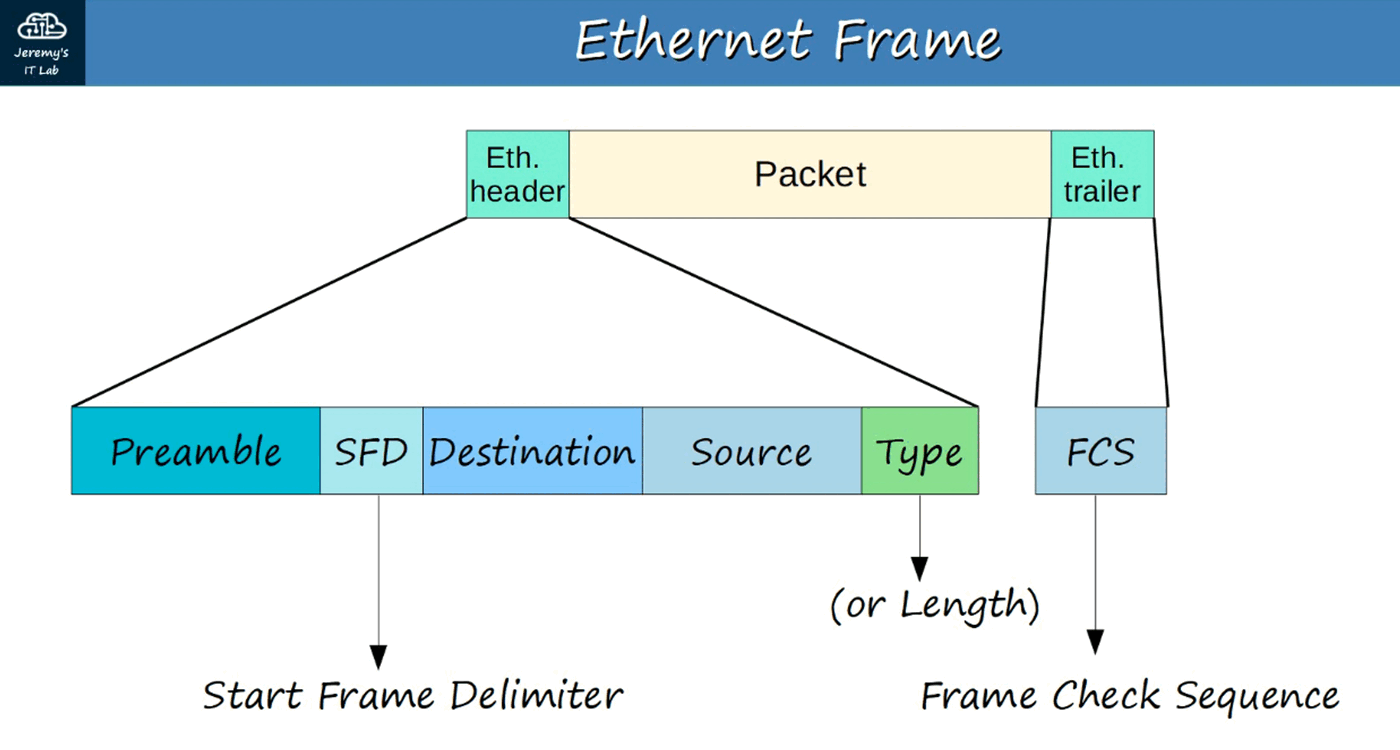
\includegraphics[keepaspectratio,alt={image}]{images/05-ethernet-lan-switching-part1/img-004.png}}
\end{figure}

Ethernet Trailer --- PACKET --- Ethernet Header

The Ethernet Header contains 5 Fields:

Preamble -- SFD -- Destination -- Source -- Type 7 bytes -- 1 byte -- 6
bytes -- 6 bytes -- 2 bytes

\section{Preamble}\label{preamble}

\begin{itemize}
\tightlist
\item
  Length: 7 bytes (56 bits)
\item
  Alternating 1's and 0's
\item
  10101010 * 7x
\item
  Allows devices to synchronize their receiver clocks
\end{itemize}

SFD : `Start Frame Delimiter'

\begin{itemize}
\tightlist
\item
  Length: 1 byte(8 bits)
\item
  10101011
\item
  Marks end of the PREAMBLE and beginning of rest of frame.
\end{itemize}

\section{Destination and Source}\label{destination-and-source}

\begin{itemize}
\tightlist
\item
  Layer 2 Address
\item
  Indicates the devices sending / receiving the frame
\item
  MAC = 'Media Access Control'
\item
  = 6 byte (48-bit) address of the physical device
\end{itemize}

\section{Type / Length}\label{type-length}

\begin{itemize}
\tightlist
\item
  2 bytes (16-bit) field
\item
  A value of 1\textbf{500 or less} in this field indicates the LENGTH of
  the encapsulated packet (in bytes)
\item
  A value of \textbf{1536 or greater} in this field indicates the TYPE
  of the encapsulated packet and length is determined via other methods.
\item
  IPv4 = 0x0800 (hexadecimal) = 2048 in decimal
\item
  IPv6 = 0x86DD (hexadecimal) = 34525 in decimal
\item
  Layer 3 protocol used in the encapsulated Packet, which is almost
  always Internet Protocol (IP) version 4 or version 6.
\end{itemize}

The ETHERNET TRAILER contains:

\section{Fcs}\label{fcs}

\begin{itemize}
\tightlist
\item
  `FRAME CHECK SEQUENCE'
\item
  4 bytes (32 bits) in length
\item
  Detects corrupted data by running a `CRC' algorithm over the received
  data
\item
  CRC = ``Cyclic Redundancy Check''
\end{itemize}

Altogether the ETHERNET FRAME = 26 bytes (header + trailer)

\begin{figure}
\centering
\pandocbounded{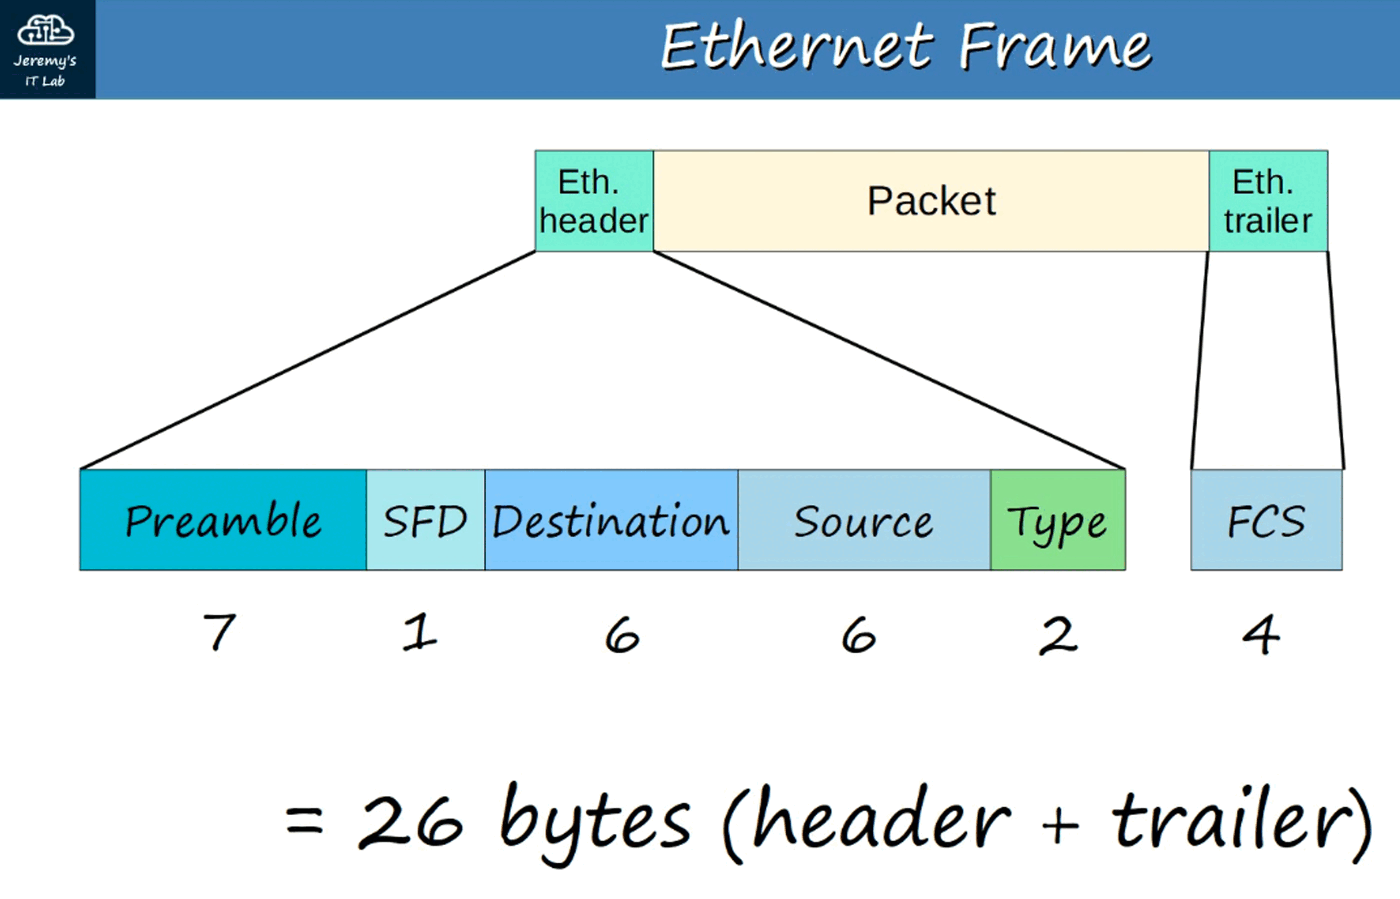
\includegraphics[keepaspectratio,alt={image}]{images/05-ethernet-lan-switching-part1/img-005.png}}
\end{figure}

MAC ADDRESS (48 bits long)

\begin{itemize}
\tightlist
\item
  6-bytes (48-bits) physical address assigned to the device when it is
  made.
\item
  AKA `Burned-In Address' (BIA)
\item
  Is globally unique
\item
  First 3 bytes are the OUI (Organizationally Unique Identifier) which
  is assigned to the company making the device
\item
  The last 3 bytes are unique to the device itself
\item
  Written as 12 hexadecimal characters
\end{itemize}

Example:

E8:BA:70 // 11:28:74 OUI // Unique Device ID

\section{Hexadecimal}\label{hexadecimal}

\begin{figure}
\centering
\pandocbounded{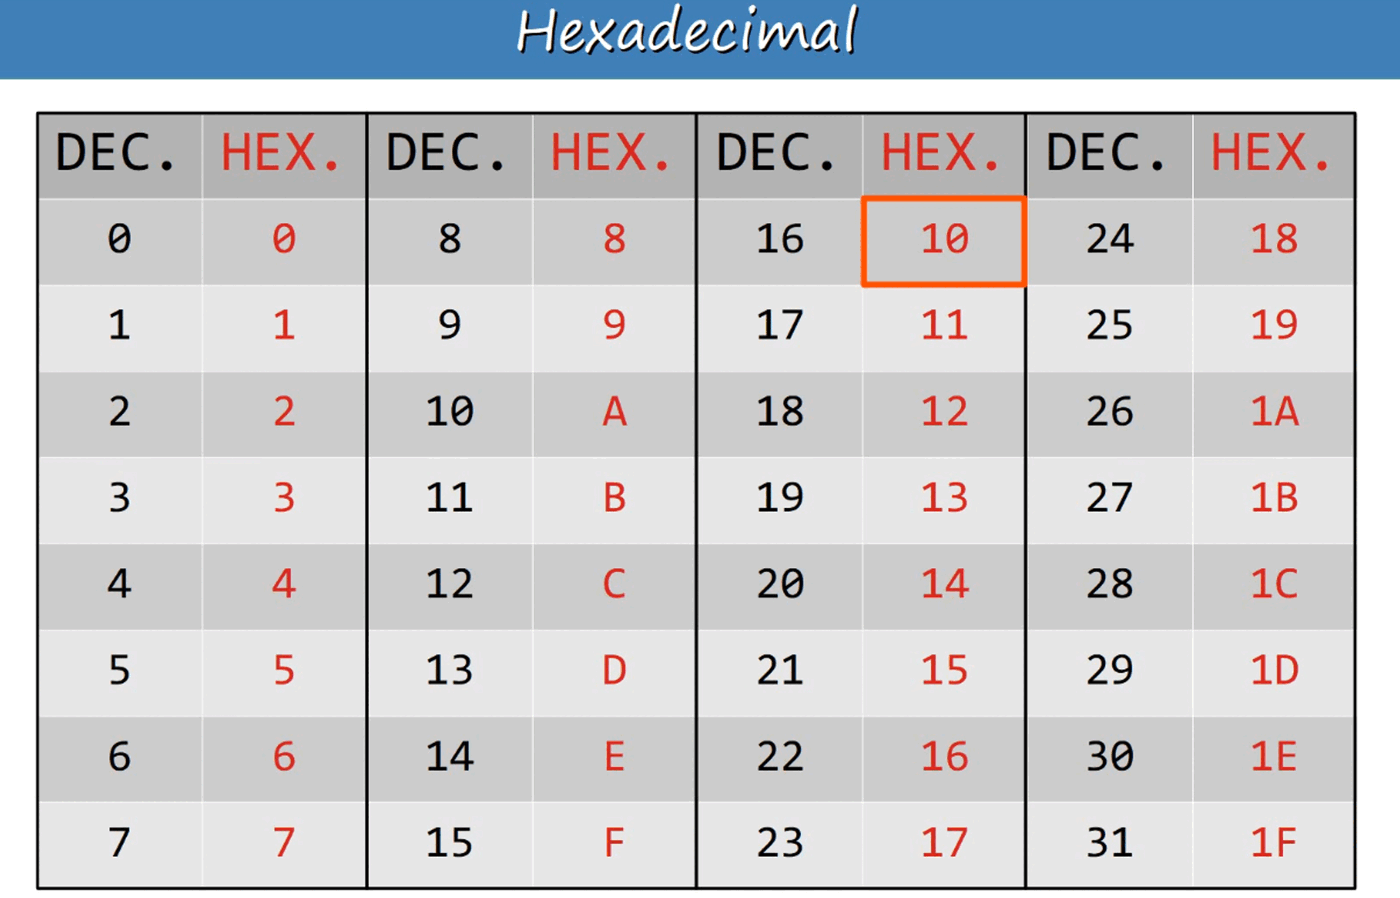
\includegraphics[keepaspectratio,alt={image}]{images/05-ethernet-lan-switching-part1/img-006.png}}
\end{figure}

\section{Interface Names}\label{interface-names}

F0/1, F0/2, F0/3\ldots{} F stands for ``Fast Ethernet'' or 100 Mbps
interfaces.

\section{MAC Address Table}\label{mac-address-table}

Each Switch stores a DYNAMICALLY LEARNED MAC ADDRESS TABLE, using the
SOURCE MAC ADDRESS of frames it receives.

\begin{figure}
\centering
\pandocbounded{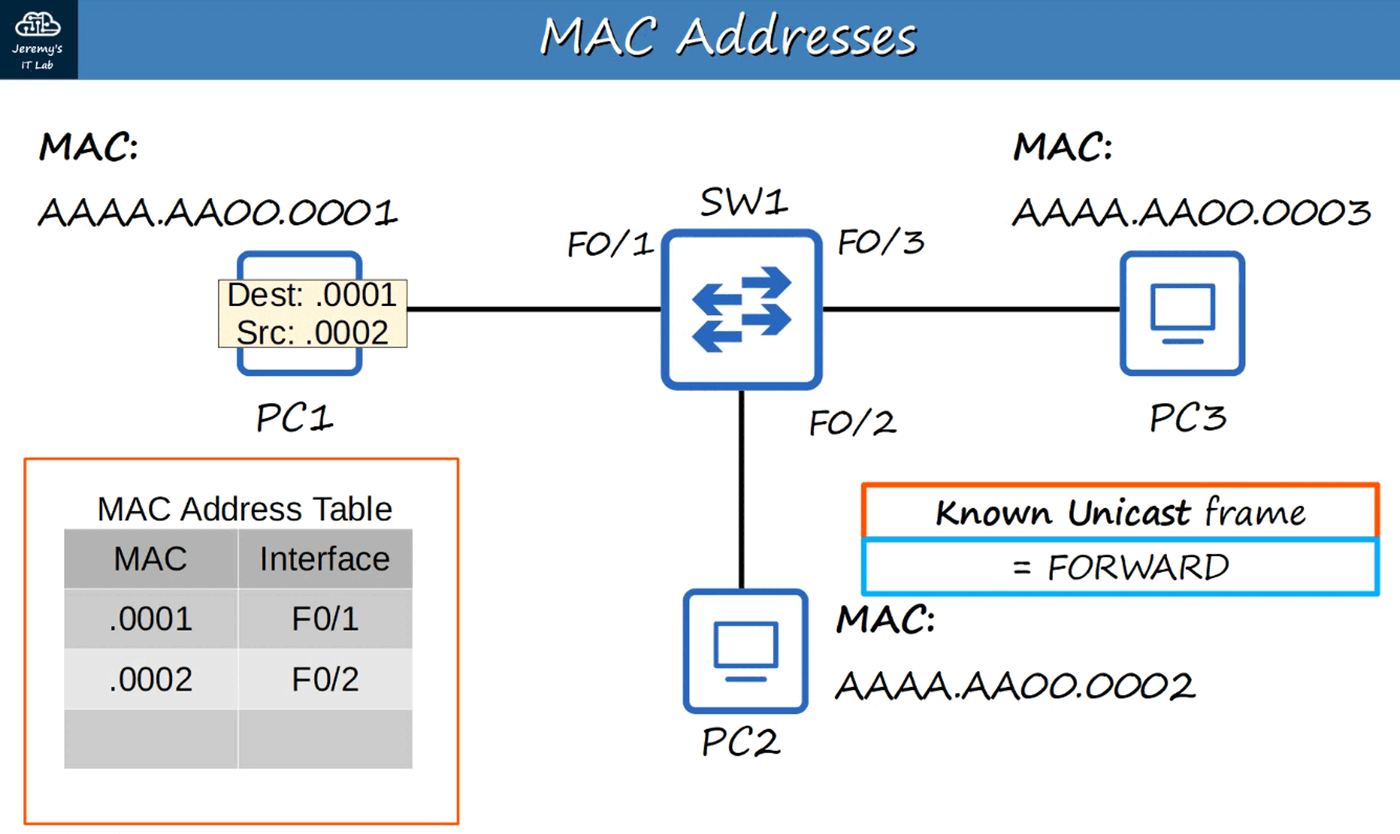
\includegraphics[keepaspectratio,alt={image}]{images/05-ethernet-lan-switching-part1/img-007.png}}
\end{figure}

When a Switch doesn't know the DESTINATION MAC ADDRESS of a frame
(UNKNOWN UNICAST FRAME), it is forced to FLOOD the frame - Forward the
frame out of ALL it's interfaces, except the one it received the packet
from.

When a KNOWN Unicast Frame is known (MAC Address is recognized by the
entry in the MAC ADDRESS TABLE), the frame is FORWARDED like normal.

\begin{figure}
\centering
\pandocbounded{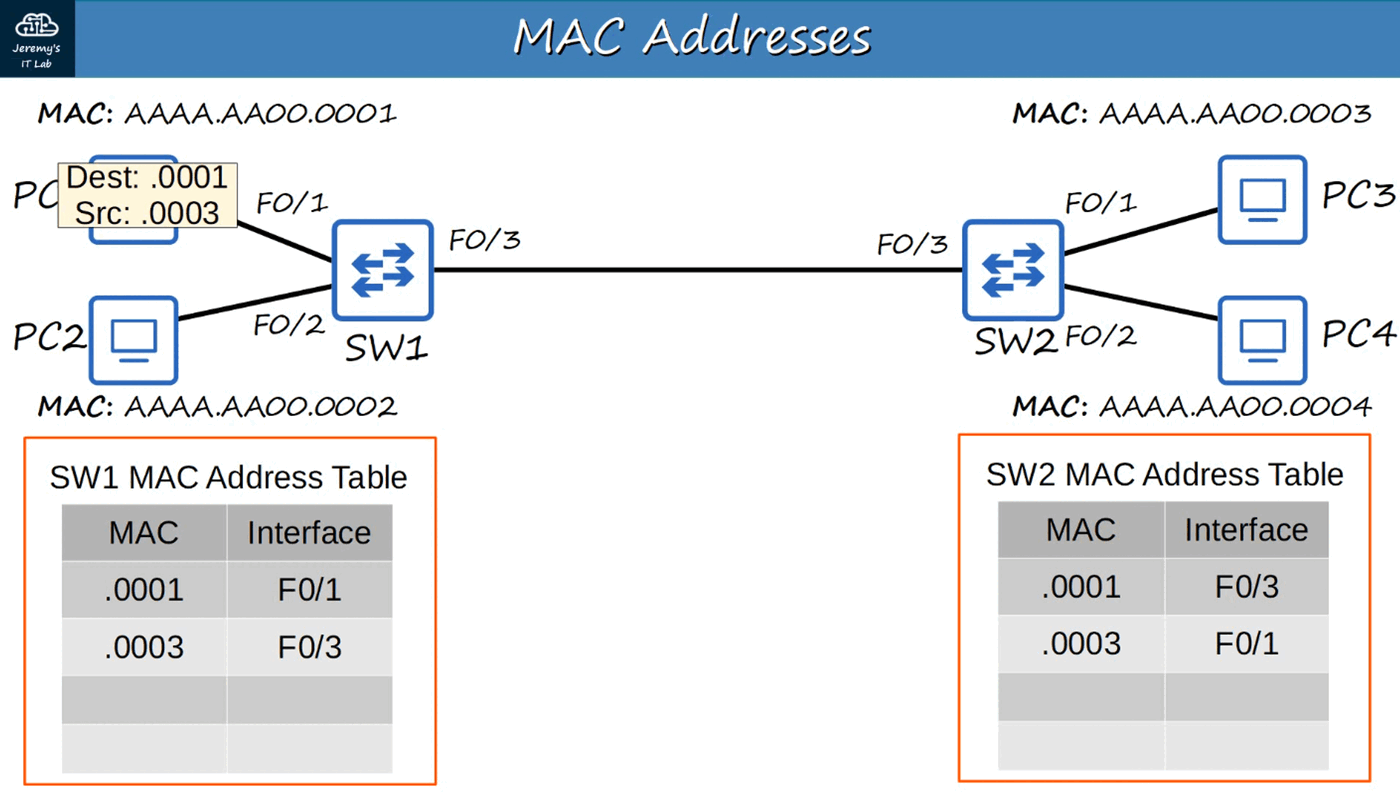
\includegraphics[keepaspectratio,alt={image}]{images/05-ethernet-lan-switching-part1/img-008.png}}
\end{figure}

\begin{itemize}
\tightlist
\item
  Note: Dynamic MAC Addresses are removed from the MAC ADDRESS TABLE
  every 5 minutes of inactivity.
\end{itemize}
